\section{SNR-Adaptive Link Modes}
\label{sec:modes}

The article's waveform operates around $-7$\,dB.  The first major
extension scales the coherent-accumulation tile factor (and the
preambles with it) into three link modes
(Table~\ref{tab:modes}), trading bitrate for sensitivity.

\begin{table}[H]
    \centering
    \caption{Link modes (sensitivities at PER $\le 10\,\%$,
             recalibrated receiver, article channel, 6\,kHz-band SNR).}
    \label{tab:modes}
    \small
    \begin{tabular}{@{}lrrrr@{}}
    \toprule
    \textbf{Mode} & \textbf{Tiles} & \textbf{ZC root} &
    \textbf{User rate (BPSK 1/3)} & \textbf{Sensitivity} \\
    \midrule
    NORMAL  & $4\times$  & 17 & 118\,bit/s & $-7.6$\,dB \\
    ROBUST  & $16\times$ & 19 & 31\,bit/s  & $-11.7$\,dB \\
    EXTREME & $64\times$ & 21 & 7.8\,bit/s & $-17.9$\,dB \\
    \bottomrule
    \end{tabular}
\end{table}

Shannon capacity~\cite{shannon1948} of the 2100\,Hz occupied band at
$-20$\,dB (6\,kHz reference) is $\approx$30\,bit/s; EXTREME's channel
rate of 22\,bit/s is 78\,\% of capacity, so the theoretical wall for
this bandwidth is $-20.7$\,dB and the measured $-17.9$\,dB floor sits
$\approx$3\,dB from it.

\subsection{What Makes the Low-SNR Modes Work}

Each of the following was found necessary empirically; removing any one
of them collapses the EXTREME mode.

\paragraph{Per-symbol residual-CFO hypothesis search.}  A $64\times$
tiled symbol integrates coherently over 0.69\,s and cannot tolerate
even a few Hz of residual CFO across the accumulation window; per-tile
phase tracking (the NORMAL-mode polynomial fit) is pure noise at
$-19$\,dB.  The tiled demodulator instead derotates the whole symbol
over a grid of frequency hypotheses, accumulates tiles under each, and
keeps the hypothesis with maximum in-band energy --- spending the
symbol's \emph{entire} energy ($\approx$19\,dB $E/N_0$ even at
$-20$\,dB SNR) on the frequency decision.  A slew-limited tracker
(full grid on the first symbol, $\pm 2$ grid steps thereafter)
suppresses per-symbol argmax noise; the search range must cover the
worst-case preamble CFO error ($\pm 25$\,Hz for EXTREME).

\paragraph{Finer detection FFT.}  ROBUST and EXTREME tone detection
uses 512-point spectrogram blocks: $4\times$ more tone energy per bin,
and a 23.4\,Hz coarse-CFO grid whose residual fits a plain lag-$N$
estimate.

\paragraph{Group-coherent ZC correlation.}  The ZC stage correlates
kernels of 2--4 concatenated ZC symbols (magnitudes summed across
groups) with a small fractional-CFO hypothesis grid ($\pm 15$\,Hz) ---
single-symbol correlation is not selective enough at $-18$\,dB, and
Section~\ref{sec:sync}'s ambiguity argument forbids a wide frequency
scan.

\paragraph{Per-mode preamble roots.}  The receiver cannot read the tile
factor from the header, because it needs the tile factor to demodulate
the header.  The mode is therefore signalled by the preamble itself:
each mode owns a distinct ZC root (17/19/21), a wrong-root matched
filter simply does not lock, and \texttt{demod\_frame\_auto} tries the
modes in turn (Figure~\ref{fig:mode_autodetect}).  Detection thresholds
were tuned against noise-only false alarms (0/20 on pure noise, all
modes).

\begin{figure}[H]
    \centering
    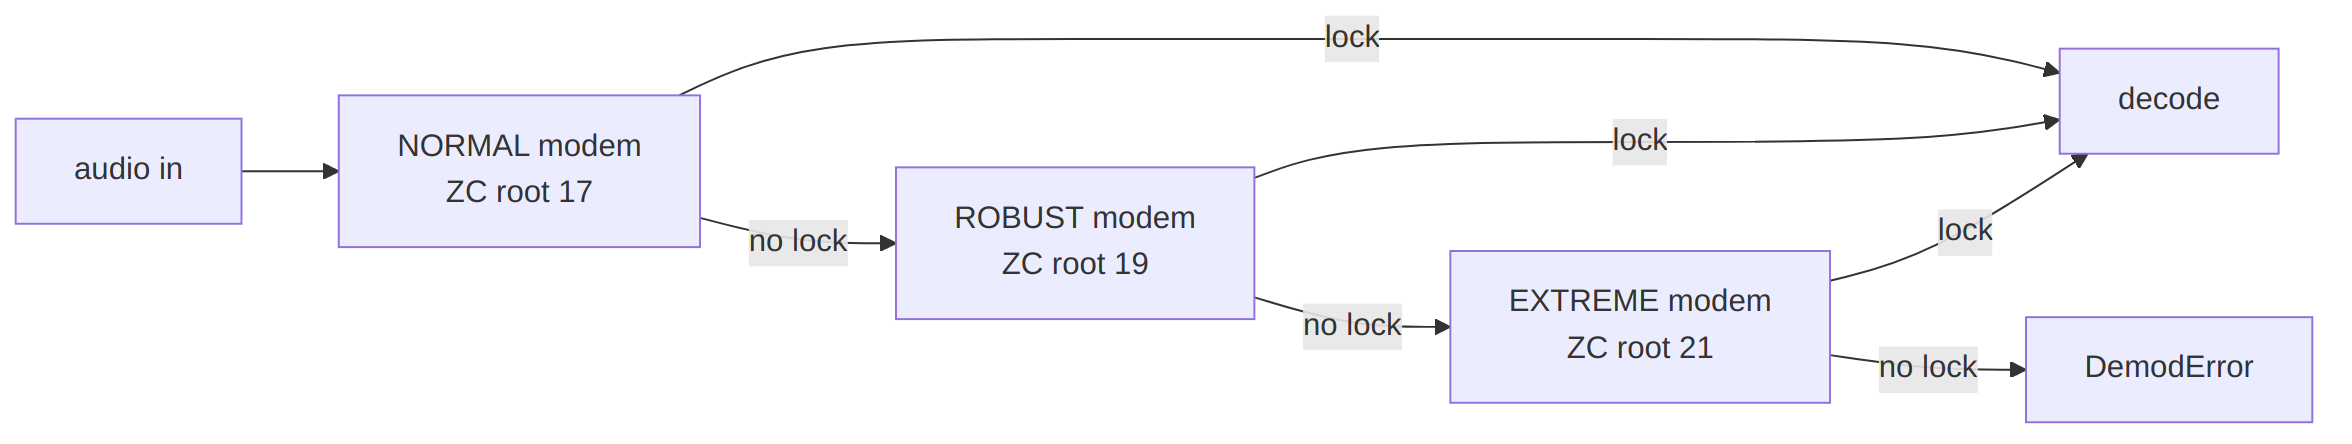
\includegraphics[width=0.9\textwidth]{images/mode_autodetect.png}
    \caption{Blind mode detection: the preamble root \emph{is} the mode
             signal.  A consequence used throughout the link layer: a
             mode switch can never deadlock the link.}
    \label{fig:mode_autodetect}
\end{figure}


\subsection{Constellations Across the Operating Range}

Figure~\ref{fig:const_ladder} makes the adaptation policy visible in
one picture: for eight SNRs spanning the whole operating range
($-17.5$ to $+20$\,dB), it shows the \emph{equalized received
constellation of the rung the rate controller actually selects} at
that SNR (highest rung whose measured sensitivity clears a 1\,dB
margin).  Each panel is produced by the real per-symbol receive chain
--- coherent tiling accumulation, per-symbol frequency search where
the mode uses one, and MMSE equalization
(\texttt{experiments/figures.py}).  At $-17.5$\,dB the EXTREME BPSK
decision variable barely emerges from the noise --- which is precisely
why rung~0 pairs $64\times$ tiling with the rate-1/3 code and soft
decisions; the QPSK quadrants firm up through the mid-ladder, and the
16-QAM grid the top rungs rely on only becomes usable above
$\approx$+3\,dB, matching the ladder sensitivities of
Table~\ref{tab:ladder}.

\begin{figure}[H]
    \centering
    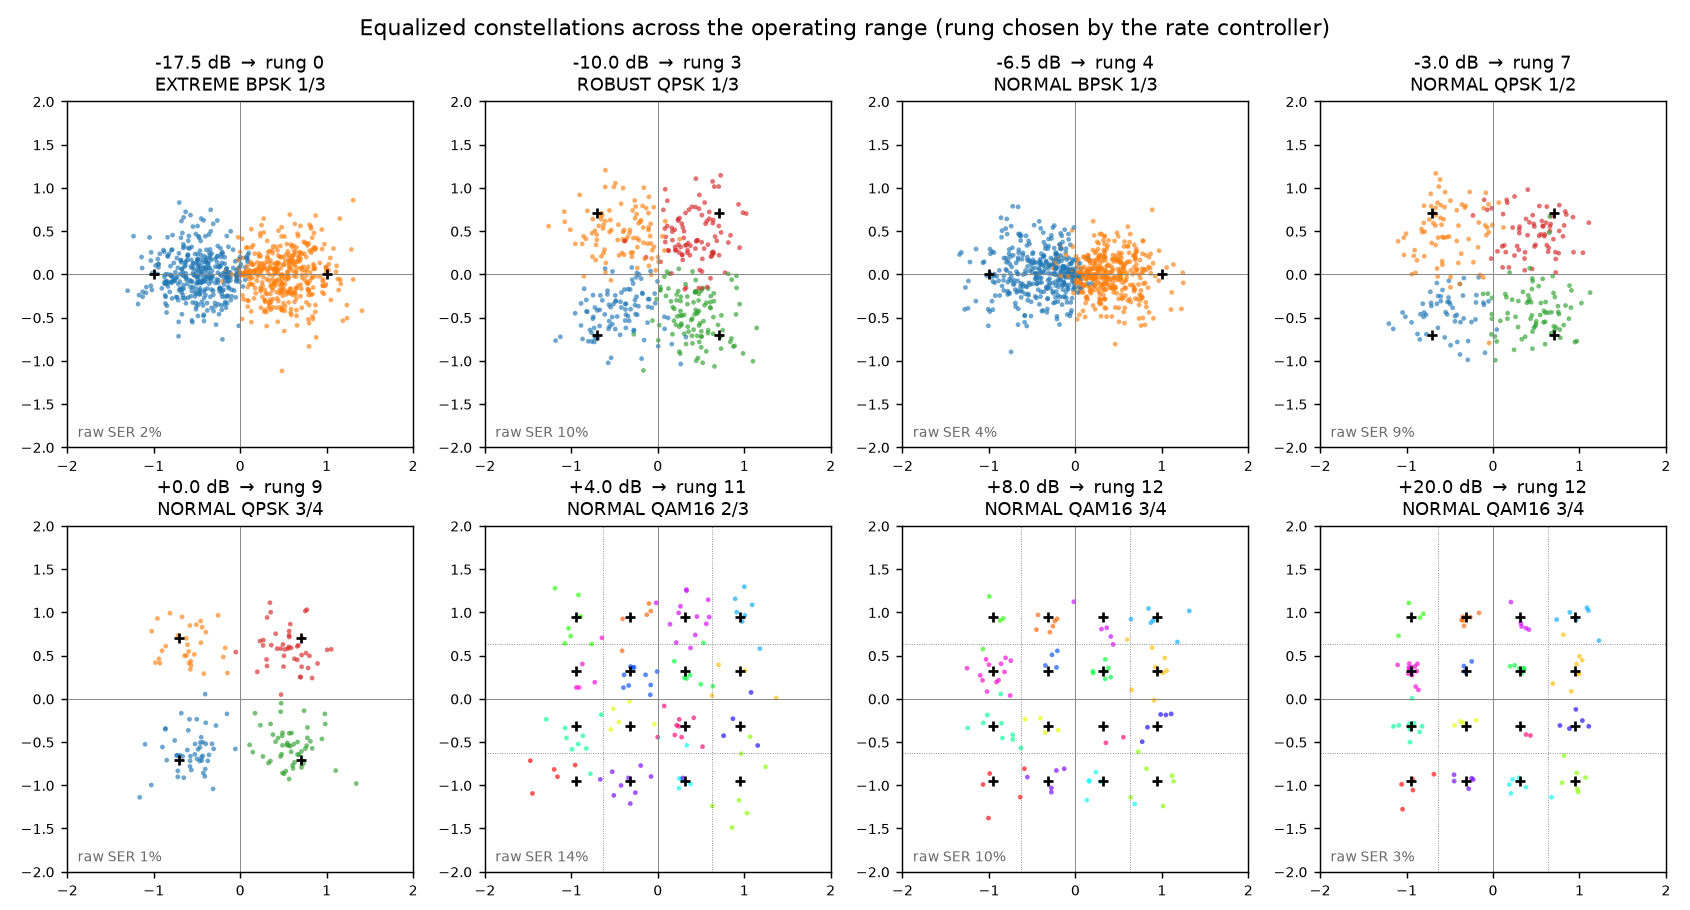
\includegraphics[width=\textwidth]{images/constellation_ladder.png}
    \caption{Equalized constellations at the controller-selected rung,
             from the EXTREME sensitivity floor to a clean channel
             (article channel, AWGN + CFO).  Black crosses mark the
             ideal constellation points; each received point is colored
             by the \emph{transmitted} symbol, so raw pre-FEC errors
             appear as points of the wrong color inside a neighbouring
             decision region (the per-panel ``raw SER'' annotation
             counts them), and the dotted subgrid on the 16-QAM panels
             marks the decision boundaries between the 16 cells.}
    \label{fig:const_ladder}
\end{figure}

\subsection{Measured Waterfalls}

Figure~\ref{fig:adaptive_modes} shows the three modes' PER waterfalls
on the article channel.  The function \texttt{select\_mode} implements
the resulting adaptation policy (mode + modulation + code rate for an
expected SNR), later subsumed by the link-layer ladder of
Section~\ref{sec:link}.

\begin{figure}[H]
    \centering
    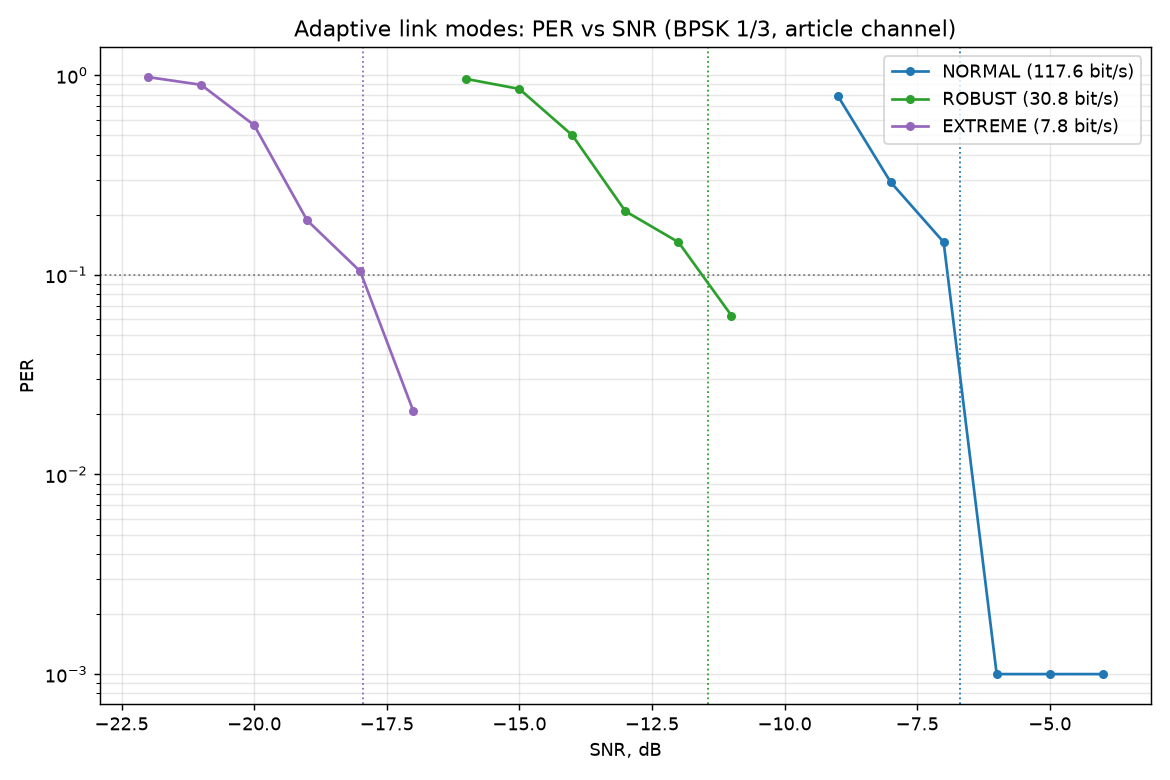
\includegraphics[width=0.9\textwidth]{images/per_adaptive_modes.png}
    \caption{PER versus SNR for the three link modes
             (\texttt{experiments/adaptive\_modes.py}).}
    \label{fig:adaptive_modes}
\end{figure}
